\documentclass[a4paper, twocolumn]{article}
\usepackage[utf8]{inputenc}
\usepackage[T1]{fontenc}
\usepackage{lmodern}
\usepackage[pdftex, hidelinks,
            pdftitle={Monte Carlo Raytracing from Scratch},
            pdfauthor={Martin Estgren and Erik S. V. Jansson},
            pdfsubject={Rendering -- Global Illumination},
            pdfkeywords={rendering, global illumination, mcrt, c,
                         path tracing, photon mapping}]{hyperref}

\usepackage{bm}
\usepackage{caption}
\usepackage{listings}
\usepackage{booktabs}
\usepackage{mathtools}
\usepackage{subcaption}
\usepackage{algorithmic}
\usepackage{graphicx}
\usepackage{courier}
\usepackage{amsmath}
\usepackage{amssymb}
\usepackage{algorithm}
\usepackage[capitalize, noabbrev]{cleveref}
\usepackage[activate={true, nocompatibility}, final,
            tracking=true, kerning=true, spacing=true,
            factor=1100, stretch=10, shrink=10]{microtype}

\DeclareCaptionFormat{modifiedlst}{\rule{\textwidth}{0.85pt}\\[-2.9pt]#1#2#3}
\captionsetup[lstlisting]{format =  modifiedlst,
labelfont=bf,singlelinecheck=off,labelsep=space}
\lstset{basicstyle=\footnotesize\ttfamily,
        breakatwhitespace = false,
        breaklines = true,
        keepspaces = true,
        language = C++,
        showspaces = false,
        showstringspaces = false,
        frame = tb,
        numbers = left,
        numbersep = 5pt,
        xleftmargin = 16pt,
        framexleftmargin = 16pt,
        belowskip = \bigskipamount,
        aboveskip = \bigskipamount,
        escapeinside={<@}{@>}}

\title{\LARGE{\textbf{Monte Carlo Raytracing from Scratch}}}
\author{{\textbf{Martin Estgren}} \;\;\;\;\;\;\;\;\;\;\;\;\;\,   {\href{mailto:mares480@student.liu.se}
                                                                 {\texttt{<mares480@student.liu.se>}}} \\
        {\textbf{Rasmus Hedin}} \;\;\;\;\;\;\;\;\;\;\;\;\;\;\,\, {\href{mailto:rashe877@student.liu.se}
                                                                 {\texttt{<rashe877@student.liu.se>}}} \\
        {\textbf{Erik S. V. Jansson}} \;\;\;\;\;\;\;\;           {\href{mailto:erija578@student.liu.se}
                                                                 {\texttt{<erija578@student.liu.se>}}} \\~\\
        {Linköping University, Sweden}\vspace{-1.0ex}}

\begin{document}
    \maketitle
    \section*{Abstract}

    \newpage \tableofcontents \clearpage

    \section{Introduction} \label{sec:introduction}

        Several fields of industry use \emph{computer graphics} to generate and display synthetic images on a screen; e.g.\ the entertainment industry uses \emph{raytracers} for \emph{rendering} animated movies while \emph{rasterizers} usually are the technology powering real-time video games. Of course, it's also widely used in the engineering and scientific disciplines for visualizing field data, which even have their own sub-field called \emph{scientific visualization}. Since it is such a wide field, we'll only be focusing on the \emph{rendering problem}: the task of converting one \emph{scene description} to an \emph{image} of it.

        Rendering can usually be done in one of two ways, called the \emph{rasterization} and \emph{raytracing} techniques, or, by using some hybrid of these. \emph{Rasterization} is when we geometrically project a scene, composed of primitives, onto an image plane (our camera) and then color the pixels based on a \emph{local lighting model}. Meaning, objects in a scene are \emph{shaded} only based on position, material properties, viewpoint direction, and light source information; never on other objects. Rasterization is very fast since there is hardware dedicated to these operations, and each of these is independent of each other, in other words, it's an \emph{embarrassingly parallel} problem. \emph{Raytracing} on the other hand shoots \emph{rays} from the pixels in the \emph{camera viewplane} and finds \emph{intersections} with geometry in the scene. These rays bounce around the scene by \emph{specular reflection} or \emph{specular transmission}, until it finds a \emph{diffuse surface}, which then \emph{absorbs} it. It's a process by recursion, which approximates \emph{irradiance} falling onto a pixel. Since it takes into account other objects, it's a technique which gives \emph{global illumination}. Unfortunately, raytracing doesn't have full hardware support, but is still fast since it's also an embarrassingly parallel task (done for each sample).

        In this report we'll describe all the party tricks we've used to implement our \emph{Monte Carlo raytracer} from scratch. It simulates all \emph{light transport} effects for \emph{perfectly diffuse} and \emph{perfectly specular} surfaces. We've also implemented \emph{photon mapping} to speed up our convergence rate for higher quality \emph{caustics}. Arbitrary \emph{triangle meshes} can also be rendered and use \emph{bounding volumes} to ignore low-effort intersection tests. Lastly, we also support \emph{quadric geometry}. All of our scene is specified by using a JSON format.

        We continue \cref{sec:introduction} by giving a brief overview of the field and introducing desirable properties for achieving \emph{photorealism} with a model describing it. We then take a excursion through the most notable rendering schemes to solve the \emph{rendering equation}. In \cref{sec:theory_and_method} we break apart our raytracer bit-by-bit and explain each part in turn, along with any relevant theory necessary. We then play around with our raytracer's knobs in \cref{sec:results_and_benchmark} to see if they affect the final render, and more importantly, the rendering time. We'll try to see if there is a balanced trade-off between render quality and speed. After all this, \cref{sec:discussion_and_outlook} concludes the report by critically looking at our implementation and results and also giving insight into what could be improved further.

    \begin{figure}[ht]
        \centering
        \begin{subfigure}{0.48\linewidth}
            \centering
            \label{fig:cornell_box_local_illumination}
            \includegraphics[width=\linewidth]{share/cornell_local_illumination.png}
            \caption{local illumination}
        \end{subfigure} \hfill
        \begin{subfigure}{0.48\linewidth}
            \centering
            \label{fig:cornell_box_global_illumination}
            \includegraphics[width=\linewidth]{share/cornell_global_illumination.png}
            \caption{global illumination}
        \end{subfigure}
        \caption{Two renders of the famous \emph{Cornell box} in our raytracer; comparing both illumination models.}
        \label{fig:cornell_box}
    \end{figure}

    \vspace{-1.5em}

    \subsection{Global\, Illumination} \label{sec:global_illumination}

    A rendering technique is deemed to be \emph{photorealistic} if, after full convergance, it exactly mimics reality. One of the most important ingredients for achieving photorealism is \emph{global illumination}. We can compare \emph{local illumination} and \emph{global illumination} by looking at \cref{fig:cornell_box}. Notice that GI (global illumination) has \emph{color bleeding}, \emph{hard and soft shadows} and \emph{caustics}. These phenomena are not possible in a local model without ``hacks'' like the \emph{shadow mapping} technique.

    \subsection{Rendering Equation} \label{sec:rendering_equation}

        A model describing most light transport phenomena is the \emph{rendering equation}, shown below, presented by \emph{James Kajiya}~\cite{kajiya1986rendering}. All of the rendering schemes are attempts at solving it. We present in the coming sections the most well known rendering techniques. \begin{align*}
            \mathcal{L}_o(\vec{x}, \hat{\omega}_o) &= \mathcal{L}_e(\vec{x}, \hat{\omega}_o) \; +\\
                                                   &+ \int_\Omega \mathcal{L}_i(\vec{x}, \hat{\omega}_i)
                                                      f_r(\vec{x}, \hat{\omega}_i, \hat{\omega}_o)
                                                      (\hat{n}_{x} \cdot \hat{\omega}_i) \, d\hat{\omega}_i
        \end{align*}

    \subsection{Radiosity} \label{sec:radiosity}
    \textit{Radiosity} for computer graphics assumes all surfaces are \emph{perfectly diffuse patches} (e.g. triangles), and builds on the concept of finding the radiance that is transferred between patches in the scene using an iterative process. Each iteration solves the equation below by reflecting radiance for each patch: \begin{equation*}
        B_i = E_i + \rho_i \sum_{j=1}^{n} F_{ij} B_j \; ,
    \end{equation*}
    where \(B_i\) is the \textit{radiosity} of \emph{patch} \(i\), \(E_i\) the \emph{emitted radiosity} by \(i\), \(\rho_i\) is the \textit{surface reflectivity} of \(i\), and the sum defines the \emph{radiance} falling onto \(i\) between each patch in the scene and the patch \(i\), depending on the \emph{form-factor} \(F_{ij}\) (geometric term) of \(i\) and \(j\).

    \begin{figure}[ht]
        \centering
        \includegraphics[width=\linewidth]{share/radiosity.png}
        \caption{Shows how the radiosity technique spreads the radiance in each iteration (render by \emph{H. Elias}).}
        \label{fig:radiosity}
    \end{figure}

    \vspace{-0.5em}

Iterating on the above equations, a discrete approximation of the \textit{rendering equation} is achieved for perfect Lambertian surfaces as the patch size goes infinitesimal and the iterations tends to infinity (but there needs to be some cutoff point, otherwise numerical errors might start appearing). You can see a radiosity-based renderer iterate through a scene in \cref{fig:radiosity}. Some advantages of radiosity over GI techniques that takes into account specular light is that it calculates the radiosity of the full scene and not just based on the camera viewport, making it useful when baking light-maps with the scene. It's a spin-off of the heat transfer equations in thermodynamics into rendering by \emph{Goral et al.}~\cite{goral1984modeling}.

    \subsection{Whitted Raytracing} \label{sec:whitted_raytracing}

    In the \emph{Whitted}~\cite{whitted1980improved} ray tracing method initial rays are emitted from the camera into the scene. The rays will intersect with objects and new reflective and/or refractive rays are spawned. In this method it is assumed that we only have \emph{perfect reflections and refractions}. The direction of a refracted ray is computed with Snell's law given the refractive indices of the materials at the ray intersection point.

    Reflecting and refracting rays will build up a \emph{tree of rays}. When all rays have terminated (i.e. hit a diffuse surface) the radiance at each intersection is computed from the leaf nodes back up to the root node (the camera). The radiance from the child rays of an intersection point contribute to the total radiance leaving each intersection point. \emph{Shadow rays} are sent from each of these points to the light sources, to know if the point is in shadow. If the shadow ray reaches a source of light then it's not in shadow and the light therefore contributes to the total radiance. \cref{fig:raytracing} (a) is being rendered by it.

    \begin{figure}[ht]
        \centering
        \begin{subfigure}{0.48\linewidth}
            \centering
            \label{fig:whitted_raytracing}
            \includegraphics[width=\linewidth]{share/whitted_raytracing.png}
            \caption{Whitted-ish raytracing}
        \end{subfigure} \hfill
        \begin{subfigure}{0.48\linewidth}
            \centering
            \label{fig:monte_carlo_raytracing}
            \includegraphics[width=\linewidth]{share/monte_carlo_raytracing.png}
            \caption{Monte Carlo raytracing}
        \end{subfigure}
        \caption{Renders of \emph{the scene} in \cref{sec:scene_description} using our raytracer in the early and later progress stages.}
        \label{fig:raytracing}
    \end{figure}

    \vspace{-1.5em}

    \subsection{Path Tracing} \label{sec:path_tracing}

    The \emph{path tracing} method works in a similar way to Whitted raytracing, but the reflections and refractions may not always perfect. Instead, when a ray intersects with an object it will be reflected in a \emph{random direction} originating from the \emph{hemisphere} at the intersection point. These rays are recursively reflected until they intersect with a light source. But since some rays never hit a light source another condition to terminate is needed. The solution is called \emph{Russian roulette}, where rays have a probability of being \emph{absorbed} at the intersection point. This gives the technique an unbiased result. A tree will be built recursively just as before, adding contribution from the child nodes and from the light sources (which may have an area now) with a local lighting model.

    This is a method that needs many \emph{samples} to converge, and thus uses \emph{Monte Carlo integration}; making the \emph{path tracing technique} a \emph{Monte Carlo raytracer}. \cref{fig:raytracing} (b) shows a render of a scene using our Monte Carlo raytracer; we have more interesting light phenomena than Whitted raytracing.

    \subsection{Photon Mapping} \label{sec:photon_mapping}

    One of the main problems with \textit{path tracing} is that it usually takes very long to \emph{converge} to a \emph{noise-less} image. To speed up the raytrace convergence, \emph{H. Jensen} proposed an algorithm where rays with low importance are approximated using a spatial map which describe how light sources deposit flux in the scene. These data-structures are called \textit{photon maps}~\cite{jensen1996global} and significantly speed up convergence of a typical \textit{path tracer} by requiring a bit more memory.

    \vspace{0.5em}

    \begin{figure}[ht]
        \centering
        \begin{subfigure}{0.478\linewidth}
            \centering
            \label{fig:cornell_box_photon_map}
            \scalebox{-1}[1]{\includegraphics[width=\linewidth]{share/photon_mapping.png}}
            \caption{direct light photon map}
        \end{subfigure} \hfill
        \begin{subfigure}{0.498\linewidth}
            \centering
            \includegraphics[width=\linewidth]{share/cornell_global_illumination.png}
            \caption{possible raytrace result}
        \end{subfigure}
        \caption{Here the flux coming from the light source is distributed as seen in (a) before we do raytracing.}
        \label{fig:photon_mapping}
    \end{figure}

    \vspace{-0.25em}

    \textit{Photon mapping} is done in two passes. The first pass is done before the \textit{path tracer} as a pre-processing step where photons are emitted from light sources and bounced around the scene in a way similar to the typical \textit{path tracer}. These photons are usually stored in a \emph{balanced kd-tree} whenever they hit a diffuse surface. The second pass is done in conjunction with the \textit{path tracer} where rays with low importance are approximated by photons stored around the terminating scene-intersection. The number of photons to consider is either calculated by a bounding sphere of fixed size or a sphere expanded until it encompasses a fixed number of photons. These photons are then used to approximate radiance at the intersection point. We'll see later in the report that our implementation uses the ``\emph{fixed sphere radiance estimation}'' approach for this.

In some cases a higher resolution secondary \textit{photon map} is used to show caustics effects since these are very expensive to do in regular \textit{path tracing}. In this case, photons are only emitted towards specular objects in the scene and in much greater numbers compared to the regular \textit{photon map}. This enables one to get detailed caustic effects cheaply and fast.

    \clearpage

    \section{Theory and Method} \label{sec:theory_and_method}

        \subsection{Scene Description} \label{sec:scene_description}

        \subsection{Ray-Surface Intersections} \label{sec:ray-surface_intersections}

        The scene can be constructed using a number of different geometric surfaces and requires different intersection test for each surface type. Common for them all is that the incomming ray is defined on the parametric formula \( \vec{o} + t \hat{d} \) where \( \vec{o} \in \mathbb{R}^3\) denotes the origin of the ray, \(t \in \mathbb{R}\) specifies a distance from the origin, and \(\hat{d} \in \mathbb{R}^3\) indicating the direction of the ray.
            
        \subsubsection{Parametric Sphere} \label{sec:parametric_sphere}
        
        Spherical objects are defined as a vector \(\vec{o} \in \mathbb{R}^3\) which denotes the origin of the sphere, and a scalar \(r\) as the radius of the sphere. Sphere - ray intersections are done using a geometric solution on the following form:

        \begin{align*}
            \vec{L} = \vec{o_{sphere}} - \vec{o_{ray}} \\
            t_{ca} = \vec{L} \cdot  \hat{d_{ray}} \\
        \end{align*}
        if \(t_{ca} < 0\), there's no intersection between ray and sphere. otherwise look for intersection points using:
        
        \begin{align*}
            d^2 = L \cdot L - t_{ca} \cdot t_{ca}
        \end{align*}
        if \(d^2 > r^2\), there's not intersection, otherwise:

        \begin{align*}
            t_{hc} &= \sqrt{r^2 - d^2} \\
            t_0 &= t_{ca} - t_{hc} \\
            t_1 &= t_{ca} + t_{hc} \\
            t_{min} &= min(t_0, t_1)
        \end{align*}
        where \(t_{min}\) is the distance from \(\vec{o_{ray}}\) to the closest intersection point on the sphere. If \(t_{min}  < 0\) we don't have an intersectino as well. The intersection point is calculataed as  \(\vec{i} = \vec{o_{ray}} + t_{min} \hat{d_{ray}} - o_{sphere} \) and the surface normal as \( \hat{n} = || \vec{i} - \vec{o_{sphere}} || \).

        \subsubsection{Triangle Polygon} \label{sec:triangle_polygon}
        
        Intersections between triangles and ray are computed using the \textit{Möller-Trumbore} algorithm which allow for intersection tests without having to compute the triangle containing plane. First a local coordinate system for the triangle is computed using the corner vertecies \(\vec{v_1}\), \(\vec{v_2}\), and \(\vec{v_3}\) on the form:

\begin{align*}
    \hat{e_1} = \vec{v_2} - \vec{v_1} \\
    \hat{e_2} = \vec{v_3} - \vec{v_1}
\end{align*}

the surface normal is extracted as \( \hat{n} =\hat{e_1} \times \hat{e_2} \)

we check if the ray travels parallel with the triangle surface by \(\hat{p} = \hat{d_{ray}} \times \hat{e_2}\), and if the determinant  \(d = \hat{e_1} \cdot \hat{p}\), \(d = 0 \), the ray does not intersect the triangle. Otherwise the intersection test continues with

\begin{align*}
    \vec{t} &= \vec{o_{ray}} - \vec{v_1} \\
    \vec{q} &= \vec{t} \times \hat{e_1} \\\\
    u &= \vec{t} \cdot \hat{p} * d^{-1} \\
    v &= \hat{d_{ray}} \cdot \vec{q} * d^{-1}
\end{align*} 
if the two conditions
 
\begin{align*}
    u < 0 \; &\textbf{and} \; u > 1 \\
    v < 0 \; &\textbf{and}  \; u + v > 1 
\end{align*}
holds we have an intersection and the distance \(t\) the ray has to travel to the intersection point can be calculated as \(\vec{e_2} \cdot \vec{q} * d^{-1} \).

        
        \subsubsection{Triangle Mesh} \label{sec:triangle_mesh}
        
        To speed up the intersection testfor geometries using mulltiple triangles we use a herarchical geometric representation where the geometry of interest is encapsulated within a bounding sphere, this allows for faster intersection tests by only having to take the triangles into account if we already know that the ray will intersect the bouding sphere.

    The bouding sphere is calcualted by picking the smallest and largest \textit{vertecies} from the vertex set \(\mathcal{V}\)
    \begin{align*} 
        \vec{v_{min}} &= \underset{\vec{v} \in \mathcal{V}}{argmin}(\vec{v}) \\
        \vec{v_{max}} &= \underset{\vec{v} \in \mathcal{V}}{argmax}(\vec{v})
    \end{align*}
    and defining the bounding sphere as:
    \begin{align*}
        radius &= \frac{ || \vec{v_{min}} - \vec{v_{max}} ||}{2} \\
        \vec{origin} &= \frac{\vec{v_{max}} - \vec{v_{min}}}{2}
    \end{align*}
 
        \clearpage

        \subsection{Surface Properties} \label{sec:surface_properties}

            After hitting a diffuse surface with normal \(\hat{n}\) coming from a ray direction \(\hat{\omega}_i\), we need to find the reflected radiance going towards \(\hat{\omega}_o\). This is affected by the \emph{bidirectional reflectance distribution function}, \(f_r\), of the surface. It's used to model the \emph{ratio} of \emph{reflected radiance} leaving the surface towards \(\hat{\omega}_o\) with respect to the \emph{irradiance} arriving from the direction \(\hat{\omega}_i\). The first definition given by \emph{F. E. Nicodemos}~\cite{nicodemus1965directional} shows: \[f_r(\vec{x}, \hat{\omega}_i, \hat{\omega}_o) = \frac{d \mathcal{L}_{r}(\vec{x}, \hat{\omega}_o)}{\mathcal{L}_i(\vec{x}, \hat{\omega}_i)(\hat{n} \cdot \hat{\omega}_i)d\hat{\omega}_i}\; .\]

            There are several \emph{surface reflectance models}; we'll only describe the \emph{Lambertian} and the \emph{Oren-Nayar} \emph{reflectance models}, since those are in our raytracer.

            \subsubsection{Lambertian Model} \label{sec:lambertian_model}

                Assumes the surface reflects radiance \emph{isotropically}, meaning it reflects radiance \emph{equally in all directions}. It was introduced by \emph{J. H. Lambert}~\cite{lambert1760photometria} in 1760, and realistically models perfectly diffuse surfaces which are free of imperfections (i.e. there is no roughness).

                \begin{figure}[ht]
                    \centering
                    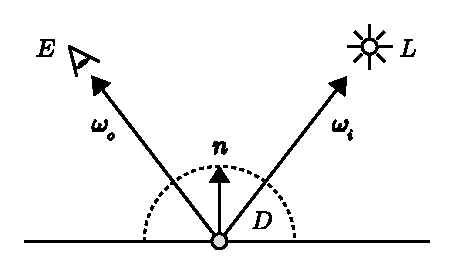
\includegraphics[width=0.8\linewidth]{share/lambertian_model.eps}
                    \caption{Diffuse ``Lambertian'' surface.}
                    \label{fig:lambertian_model}
                \end{figure}

                Since it doesn't depend on the incoming/outgoing directions, the value of \(f_r\) is constant in all directions within the hemisphere. This gives us the BRDF in \cref{eq:lambertian_model}. Now, usually you see the factor \(\hat{n} \cdot \hat{\omega}_i\) here as well, but we've chosen to not include it since it'll be appearing in the rendering equation anyway.

                \begin{equation} \label{eq:lambertian_model}
                    f_r(\vec{x}, \hat{\omega}_i, \hat{\omega}_o) = \frac{\rho}{\pi} \; ,
                \end{equation} where \(\rho\) is the \emph{albedo} of the diffuse surface \(D\) and \(\pi\) is the \emph{normalization factor} for \emph{energy conservation}. \emph{Albedo} can hand-wavingly be interpreted as ``color''.

            \subsubsection{Oren-Nayar Model} \label{sec:oren-nayar_model}

                Unfortunately, while the Lambertian model might be good for some surface types, it's inappropriate for others, such as concrete, ceramic and cloth. Which is a shame, since it's an simple and intuitive model.

                Surfaces which are diffuse and have rough texture can be accurately modeled with the \emph{Oren-Nayar}~\cite{oren1994generalization} \emph{reflection model}. It's based on the \emph{microfacet model} introduced by \emph{Torrace-Sparrow}~\cite{torrance1967theory}, which assumes a surface is composed of infinitesimally small, flat, Lambertian reflectors (as shown in the last section). An intuitive sketch of such a surface can be seen in \cref{fig:oren-nayar_model}, where the V-shaped microfacets are actually supposed to be infinitesimally small sized.

                \begin{figure}[H]
                    \centering
                    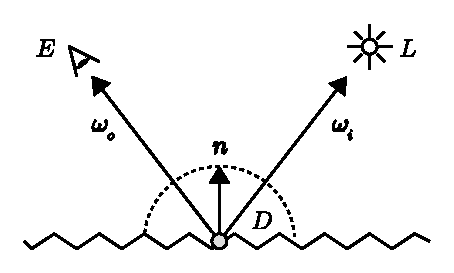
\includegraphics[width=0.8\linewidth]{share/oren-nayar_model.eps}
                    \caption{Diffuse ``Oren-Nayar'' surface.}
                    \label{fig:oren-nayar_model}
                \end{figure}

                Deriving \cref{eq:oren-nayar_model} is outside the scope of this paper, so if you're interested, consult the original paper. Note that this is the \emph{qualitative Oren-Nayar} definition, and will therefore fail energy conservation laws when the \emph{roughness} parameter is set \(\sigma > 0.97\).

                \begin{equation} \label{eq:oren-nayar_model}
                    \begin{split}
                        f_r(\vec{x}, \hat{\omega}_i, \hat{\omega}_o) = \frac{\rho}{\pi} \cdot (A + \sin\alpha \cdot \tan\beta \cdot \gamma \cdot B) \; ,\\
                        A = 1 - 0.5 \frac{\sigma^2}{\sigma^2 + 0.33} \; , \; B = 0.45\frac{\sigma^2}{\sigma^2 + 0.09} \; ,\\
                        \alpha = \max\, \{\theta_i, \theta_o\} \; , \; \beta = \min\, \{\theta_i, \theta_o\} \; ,\\
                        \gamma = \max\, \{0, \phi_i - \phi_o\} \; ,
                    \end{split}
                \end{equation} where \(\theta\) is the \emph{inclination} and \(\phi\) the \emph{azimuth} of \(\hat{\omega}\). By changing \(\sigma\) we can control the \emph{surfaces' roughness}. Notice that this BRDF dependents on the ray angle, and is therefore \emph{anisotropic}. Implementing this isn't that straightforward since our raytracer has \(\hat{\omega}\)'s that aren't easily decomposable into the form \(\hat{\omega} = (\theta, \phi)\). It boils down to doing projections onto the surface plane. We can get a vector parallel to the plane with \(\hat{p} = \hat{\omega}_i \times \hat{\omega}_o\) and then \(\hat{q} = \hat{p} \times \hat{n}\). By projecting down \(\hat{\omega}_i\) onto \(\hat{q}\) with \(\hat{\omega}_{i\parallel \hat{q}}\), we get \(\theta = \hat{\omega}_i \cdot \hat{q} \; , \; \phi = \hat{\omega}_{i\parallel \hat{q}} \cdot \hat{q}\).

                Because the qualitative Oren-Nayar calculations have quite a few expensive operations, we've chosen to implement \emph{Yasuhiro Fujii's}~\cite{fujii2015improvement} Oren-Nayar variant. It doesn't require trigonometric functions, and gives empirically almost indistinguishable results to O-N. Like regular Oren-Nayar, it suffers from not following energy conservation laws when \(\sigma' > 0.97\).

                Actually, experimentally, \emph{Y. Fujii} has found that his proposed approach matches regular Oren-Nayar better than the qualitative Oren-Nayar found in \cite{oren1994generalization}.

                \vspace{-1em}

                \begin{equation} \label{eq:improved_oren-nayar_model}
                    \begin{split}
                        f_r(\vec{x}, \hat{\omega}_i, \hat{\omega}_o) = \rho \cdot \Big(A' + \frac{s}{t} \cdot B'\Big) \; ,\\
                        A' = \frac{1}{\pi + \big(\frac{\pi}{2} - \frac{2}{3}\big) \sigma'} \; , \; B' = \frac{\sigma'}{\pi + \big(\frac{\pi}{2} - \frac{2}{3}\big) \sigma'} \; ,\\
                        t = \begin{cases}
                            1 & \textbf{if}\;\;\; s \leq 0\\
                            \max\, \{\hat{n} \cdot \hat{\omega}_i, \hat{n} \cdot \hat{\omega}_o\} & \textbf{otherwise}
                        \end{cases} \; ,\\
                        s = \hat{\omega}_i \cdot \hat{\omega}_o - (\hat{n} \cdot \hat{\omega}_i)(\hat{n} \cdot \hat{\omega}_o) \; .
                    \end{split}
                \end{equation}

                Unlike qualitative Oren-Nayar, the above BRDF is a breeze to evaluate, for both the hardware and the programmer (who likes projecting stuff anyway).

                Looking at \cref{fig:roughness} we see results returned from our raytracer. We should make a couple of interesting observations. Notice that Oren-Nayar reflectors with \(\sigma' = 0\) are essentially the same as Lambertian reflectors. Which makes sense, since \(\sigma' = 0\) means the surface has no roughness (i.e. perfectly diffuse).

                \begin{figure}[ht]
                    \centering
                    \includegraphics[width=\linewidth]{share/roughness.png}
                    \caption{Spheres rendered using our raytracer with different roughness values, \(\sigma'\), for the Oren-Nayars.}
                    \label{fig:roughness}
                \end{figure}

                To wrap things up, when we hit a diffuse surface, we wish to know the ratio of radiance that will leave the surface. For this we need to choose between the Lambertian and Oren-Nayar model to calculate \(f_r\). Each surface in our scene defs. it's \(f_r\) model to use.

                \clearpage

        \subsection{Direct Light Contributions} \label{sec:direct_light_contributions}
        Most importance rays that are sent from the camera into the scene never hit a light source. Therefore, the direct light from the light sources to an intesection point needs to contribute to the total radiance at the point. This is computed with shadow rays that are sent from each intersection point to the light sources. The shadow rays will provide light which contribute to the radiance at the ray intersection points. To determine if the intersection point lies in shadow a visbility test is performed. Transparent objects are ignored by the visibility test.
            \subsubsection{Point Light Source} \label{sec:point_light_source}
            The shadow ray $S_2 = x - y$ from an intersection point $y$ to a point light source position $x$ is launched. If it does not hit any object it pass the visibility test and the light will contribute to the radiance. A falloff based on the angle $\theta_{S_2}$ between the normal $N$ and $S_2$ is applied which can be seen in the equation below.

            \begin{equation*}
              L(y \rightarrow -\Psi_1) = f_r(y, \omega_{S_2}, -\Psi_1) L(y \leftarrow S_2) cos\theta_{S_2}
            \end{equation*}
            
            \begin{figure}[ht]
              \centering
              \includegraphics[width=\linewidth]{share/point_light.png}
              \caption{Point light shadow ray}
              %\label{fig:roughness}
            \end{figure}

            \subsubsection{Area Light Source} \label{sec:area_light_source}
            The direct light from an area light source needs to be approxmiated for each intersection point. This is done with a Monte-Carlo estimator $<L_D>$ using $M$ shadow photons which will be explained in the next section. The light source is a triangle with corners $\mathbf{v_0}$, $\mathbf{v_1}$, and $\mathbf{v_2}$ and with area $A = 0.5 ||(\mathbf{v_1} - \mathbf{v_0})\times(\mathbf{v_2}-\mathbf{v_0})||$. To get the shadow rays we need to pick random points $q$ on the light source uniformely with PDF $p(q) = \frac{1}{A}$. This is done by drawing two random numbers $u, v$ until $u + v < 1$ and building the point $q$ with barycentric coordinates $q = (1-u-v)\mathbf{v_0} + u\mathbf{v_1} + v\mathbf{v_2}$. Repeat this until we have $M$ points. 


            \subsubsection{Monte Carlo Method} \label{sec:monte_carlo_method}
            \begin{equation*}
              <L_D> = \frac{AL_0}{M}\sum_{i=1}^{M}{f_r V(x, q) G(x, q_i)}
            \end{equation*}
             $G(x, q) = cos\alpha cos\beta / d^2$ is the geometric term where d is the length of the shadow ray and $\alpha$, $\beta$ are the inclination angles to the surface normal at the start- and endpoint. $V(x, q_i)$ is the visibility function which is 1 if no object is in the way and 0 otherwise. Thus, only unblocked shadow rays will contribute to the estimate giving a soft shadow. Since the light source is a Lambertian emittor $L_0$ is emitted for all points and directions of the light source.
            
            \subsection{Indirect Light Contributions} \label{sec:indirect_light_contributions}
            When rays are emitted from the camera they will intersect with surfaces. At the intersections the rays will either terminate or spawn new rays depending on the surface material. By following the path of the ray we build up a tree with intersections as nodes connected by rays. The child nodes will contribute radiance to the parent nodes which gives indirect light, i.e. light reflected at least once since it left the light source.
            \subsubsection{Specular Reflection} \label{sec:specular_reflection}
            If a ray hits a specular surface a new ray will always spawn. The direction of the new ray is determined by the perfect specular reflection law. The direction of the new ray $\vec{R} = \vec{I} - 2 (\vec{I} \cdot \vec{N}) \vec{N}$ where $\vec{I}$ is the incoming ray and $\vec{N}$ is the surface normal.

            \subsubsection{Specular Refraction} \label{sec:specular_refraction}
            If a ray hits a refractive surface, i.e. a transparent object, a new ray is spawned that enters the object.
            The refractive ray $\vec{T}$ is computed with the perfect refraction law and the angle to the surface normal is computed with \emph{Snell's law}.

            \small
            \begin{equation*}
              \vec{T} = \tfrac{n_1}{n_2}\vec{I} + \vec{N}\left(-\tfrac{n_1}{n_2}(\vec{N}\cdot\vec{I}) - \sqrt{1 - [\tfrac{n_1}{n_2}]^2[1 - (\vec{N}\cdot\vec{I})^2]}\right)
            \end{equation*}
            \normalsize

            When a ray is moving between media of different refractive indices we might both reflect and refract. The fresnel equation is used to determine the distribution of the radiance over the refracted and reflected rays.

            \begin{equation*}
            R_s = \left[\frac{n_1cos\theta_1 - n_2\sqrt{1-([n_1/n_2]sin\theta_1)^2}}{n_1cos\theta_1 + n_2\sqrt{1-([n_1/n_2]sin\theta_1)^2}}\right]^2
          \end{equation*}

          \begin{equation*}
            R_p = \left[\frac{n_2\sqrt{1-([n_1/n_2]sin\theta_1)^2} - n_1cos\theta_1}{n_2\sqrt{1-([n_1/n_2]sin\theta_1)^2} + n_1cos\theta_1}\right]^2
          \end{equation*}

          The total reflection coefficient becomes
          \begin{equation*}
            k_r = (R_s + R_p)/2
          \end{equation*}

          The radiance of the parent node to the refracted and reflected ray is computed as
          \begin{equation*}
            L = R k_r + T (1-k_r)
          \end{equation*}

          \subsubsection{Diffuse Reflection} \label{sec:diffuse_refraction}
          As described in \ref{sec:surface_properties} two diffuse surfaces are implemented in the project; Lambertian and Oren-Nayar. When these surfaces are intersected by a ray we need to determine the direction of the reflected ray. For specular surfaces the ray was reflected/refracted perfectly, but for diffuse surfaces this is not the case. Instead, a random azimuth angle $\phi_i$ and inclination angle $\theta_i$ is picked in the hemisphere. We pick two random values $u, v \in [0,1)$ and compute azimuth $\phi_i = 2\pi u$ and inclination $\theta_i = cos^{-1}(\sqrt{v})$. The reflected ray will contribute to the radiance at the intersection giving indirect light.

          In order to not get a biased result an unbiased termination condition is required. This is achieved with russian roulette \ref{sec:russian_roulette} that determines if a ray should be terminated.

          \subsubsection{Russian Roulette} \label{sec:russian_roulette}
          In order to achieve a unbiased result russian roulette is used to get an unbiased termination condition. The idea is to select a reflection probabilty $P$ for an intersection of a ray. This probability is connected to the surface properties. The radiance at a intersection point is approximated with a Monte-Carlo scheme using one ray.

          \begin{equation*}
            L(x \rightarrow \omega_{out}) = \pi f_r(x, \omega_{in}, \omega_{out}) L(x \leftarrow \omega_{in})
          \end{equation*}

          A new ray is spawned at the intersection point with probability $P$ and the ray is terminated with probability $(1-P)$. In order to remove the bias the following equation is used.

          \begin{equation*}
            L(x \rightarrow \omega_{out}) = \frac{\pi}{P} f_r(x, \omega_{in}, \omega_{out}) L(x \leftarrow \omega_{in})
          \end{equation*}

          To determine if a ray should be terminated the azimuth angle of the reflected ray is modified to $\phi_i = (2\pi/P)u$ where $u$ is a random variable $0 \leq u \leq 1$. If $\phi_i > 2\pi$ the ray is terminated and a new ray is spawned if $0 \leq \phi_i \leq 2\pi$.
        \subsection{Photon Mapping} \label{sec:photon_mapping}
            \subsubsection{Gathering Photons} \label{sec:gathering_photons}
            \subsubsection{Radiance Estimate} \label{sec:radiance_estimate}

        \subsection{Anti-Aliasing} \label{sec:anti-aliasing}

    \section{Results and Benchmark} \label{sec:results_and_benchmark}

    \section{Discussion and Outlook} \label{sec:discussion_and_outlook}

    \newpage % Next column...
    \nocite{*} % Include all.
    \bibliographystyle{abbrv}
    \bibliography{mcrt}
\end{document}
